\documentclass{beamer}
% =============================================================================
% ENCODING
% =============================================================================
\usepackage[utf8]{inputenc}  % UTF-8 encoding support

% =============================================================================
% GRAPHICS
% =============================================================================
\usepackage{graphicx}  % For \includegraphics (401 uses across lectures)

% =============================================================================
% MATH PACKAGES
% =============================================================================
\usepackage{amsmath}    % For align, multline, equation environments (heavily used)
\usepackage{amsfonts}   % For \mathbb (e.g., \bbR, \bbE)
\usepackage{amssymb}    % For additional math symbols

% =============================================================================
% TABLES
% =============================================================================
\usepackage{booktabs}   % For \toprule, \midrule, \bottomrule (used in lecture13, lecture14)

% =============================================================================
% LISTS
% =============================================================================
\usepackage{enumerate}  % Enhanced enumerate environment (76 uses across lectures)

% =============================================================================
% TIKZ (DIAGRAMS)
% =============================================================================
\usepackage{tikz}       % For taxonomy diagram and footnotes positioning

% =============================================================================
% UTILITY PACKAGES
% =============================================================================
\usepackage{multido}    % For \multido command used in \eqpause
\usepackage{etoolbox}   % For \AtEndEnvironment, \ifbool, \newbool (used in preamble and taxonomy)

% =============================================================================
% BEAMER THEME SETTINGS
% =============================================================================
\usetheme{default}
\usecolortheme{default}

\setbeamerfont{title}{size=\Huge}
\setbeamertemplate{footline}[frame number]{}
\setbeamertemplate{section in toc}[sections numbered]

\makeatletter
\newcommand\HUGE{\@setfontsize\Huge{35}{40}}
\makeatother    

\setbeamerfont{title}{size=\HUGE}
\beamertemplatenavigationsymbolsempty

% =============================================================================
% TIKZ LIBRARIES
% =============================================================================
% Used for taxonomy diagram: arrows, positioning, shapes
\usetikzlibrary{arrows.meta,calc,shapes,positioning,shadows,trees}

% =============================================================================
% CUSTOM FOOTNOTE COMMANDS
% =============================================================================
% \myfootnote{text} - creates a footnote at the bottom of the slide
\newcommand\myfootnote[1]{%
  \vspace{-0.5cm}%
  \tikz[remember picture,overlay]
  \draw (current page.south west) +(1in + \oddsidemargin,0.5em)
  node[anchor=south west,inner sep=0pt]{\parbox{\textwidth}{%
      \rlap{\rule{10em}{0.4pt}}\raggedright\scriptsize \textit{#1}}};}

% \myfootnotewithlink{url}{text} - creates a clickable footnote (623 uses across lectures)
\newcommand\myfootnotewithlink[2]{%
  \vspace{-0.5cm}%
  \tikz[remember picture,overlay]
  \draw (current page.south west) +(1in + \oddsidemargin,0.5em)
  node[anchor=south west,inner sep=0pt]{\parbox{\textwidth}{%
      \rlap{\rule{10em}{0.4pt}}\raggedright\scriptsize\href{#1}{\textit{#2}}}};}

% =============================================================================
% SECTION/SUBSECTION OUTLINE AUTOMATION
% =============================================================================
% Automatically show outline at the beginning of each section
\AtBeginSection[]
      {
      	\begin{frame}{Outline}
      		\tableofcontents[currentsection]
      	\end{frame}
      }
      \AtBeginSubsection[]{
      	\begin{frame}{Outline}
      		\tableofcontents[currentsection,currentsubsection]
      	\end{frame}
}

% =============================================================================
% CUSTOM SLIDE ANIMATION COMMANDS
% =============================================================================
% These commands enable step-by-step reveal of equations and content
% Used heavily across all lectures (1130+ uses of \nextonslide and \eqpause)

\newcounter{noscounter}   % Counter for \nextonslide (resets on each new slide)
\newcounter{pcounter}     % Counter for pause commands (resets after \eqpause)
\newcounter{diffcounter}  % Counts pauses after equations

% \nextonslide{content} - reveals content on the next overlay
\newcommand{\nextonslide}[1]{%
  \stepcounter{noscounter}%
  \stepcounter{pcounter}%
  \stepcounter{diffcounter}%
  \onslide<\value{noscounter}->{#1}%
}

% \resetonslide - resets all animation counters (called at each frame)
\newcommand{\resetonslide}{%
    \setcounter{noscounter}{1}%
    \setcounter{pcounter}{1}%
    \setcounter{diffcounter}{0}%
}

% \eqpause - pause after equation that syncs with \nextonslide
\newcommand{\eqpause}{%
  \multido{\i=1+1}{\value{pcounter}}{\pause}%
  \stepcounter{noscounter}%
  \setcounter{pcounter}{1}%
}

% \eqpausediff - helper command, runs automatically after math environments
\newcommand{\eqpausediff}{%
  \multido{\i=1+1}{\value{diffcounter}}{\pause}%
  \addtocounter{pcounter}{-\value{diffcounter}}%
  \setcounter{diffcounter}{0}%
}

% Apply \eqpausediff after math environments
\newcommand\AtEndBoth[2]{%
  \AtEndEnvironment{#1}{#2}%
  \AtEndEnvironment{#1*}{#2}%
}

\AtEndBoth{align}{\eqpausediff}
\AtEndBoth{equation}{\eqpausediff}
\AtEndBoth{multline}{\eqpausediff}

% Reset counters at the beginning of each frame
\addtobeamertemplate{frametitle}{\resetonslide}{}

% =============================================================================
% INCLUDE OTHER CONFIGURATION FILES
% =============================================================================
% ==============================================================================
% Custom LaTeX Commands for Deep Generative Models Course
% ==============================================================================

% ==============================================================================
% BOLD LETTERS (mathbf / boldsymbol)
% ==============================================================================

% ------------------------------------------------------------------------------
% Latin Bold Lowercase
% Usage: \bx for x in bold, commonly used for vectors
% ------------------------------------------------------------------------------
\newcommand{\ba}{\mathbf{a}}
\newcommand{\bc}{\mathbf{c}}
\newcommand{\be}{\mathbf{e}}
\newcommand{\bff}{\mathbf{f}}  % Note: \bf is reserved for bold font switching
\newcommand{\bg}{\mathbf{g}}
\newcommand{\bh}{\mathbf{h}}
\newcommand{\bp}{\mathbf{p}}
\newcommand{\bq}{\mathbf{q}}
\newcommand{\bs}{\mathbf{s}}
\newcommand{\bt}{\mathbf{t}}
\newcommand{\bu}{\mathbf{u}}
\newcommand{\bv}{\mathbf{v}}
\newcommand{\bw}{\mathbf{w}}
\newcommand{\bx}{\mathbf{x}}
\newcommand{\by}{\mathbf{y}}
\newcommand{\bz}{\mathbf{z}}

% ------------------------------------------------------------------------------
% Latin Bold Uppercase
% Usage: \bX for X in bold, commonly used for matrices or random vectors
% ------------------------------------------------------------------------------
\newcommand{\bA}{\mathbf{A}}
\newcommand{\bG}{\mathbf{G}}
\newcommand{\bI}{\mathbf{I}}
\newcommand{\bJ}{\mathbf{J}}
\newcommand{\bL}{\mathbf{L}}
\newcommand{\bM}{\mathbf{M}}
\newcommand{\bP}{\mathbf{P}}
\newcommand{\bQ}{\mathbf{Q}}
\newcommand{\bR}{\mathbf{R}}
\newcommand{\bT}{\mathbf{T}}
\newcommand{\bU}{\mathbf{U}}
\newcommand{\bV}{\mathbf{V}}
\newcommand{\bW}{\mathbf{W}}
\newcommand{\bX}{\mathbf{X}}
\newcommand{\bZ}{\mathbf{Z}}

% ------------------------------------------------------------------------------
% Greek Bold Lowercase
% Usage: \btheta for θ in bold, commonly used for parameter vectors
% ------------------------------------------------------------------------------
\newcommand{\bepsilon}{\boldsymbol{\epsilon}}
\newcommand{\blambda}{\boldsymbol{\lambda}}
\newcommand{\bmu}{\boldsymbol{\mu}}
\newcommand{\bphi}{\boldsymbol{\phi}}
\newcommand{\bpi}{\boldsymbol{\pi}}
\newcommand{\bpsi}{\boldsymbol{\psi}}
\newcommand{\bsigma}{\boldsymbol{\sigma}}
\newcommand{\btheta}{\boldsymbol{\theta}}

% ------------------------------------------------------------------------------
% Greek Bold Uppercase
% Usage: \bSigma for Σ in bold, commonly used for covariance matrices
% ------------------------------------------------------------------------------
\newcommand{\bSigma}{\boldsymbol{\Sigma}}
\newcommand{\bTheta}{\boldsymbol{\Theta}}

% ==============================================================================
% CALLIGRAPHIC LETTERS (mathcal)
% Usage: \cX for calligraphic X, commonly used for sets and spaces
% ==============================================================================
\newcommand{\cF}{\mathcal{F}}
\newcommand{\cI}{\mathcal{I}}
\newcommand{\cL}{\mathcal{L}}
\newcommand{\cM}{\mathcal{M}}
\newcommand{\cN}{\mathcal{N}}
\newcommand{\cP}{\mathcal{P}}
\newcommand{\cS}{\mathcal{S}}
\newcommand{\cT}{\mathcal{T}}
\newcommand{\cW}{\mathcal{W}}
\newcommand{\cX}{\mathcal{X}}
\newcommand{\cZ}{\mathcal{Z}}

% ==============================================================================
% BLACKBOARD BOLD LETTERS (mathbb)
% Usage: \bbR for ℝ, commonly used for number sets and expectations
% ==============================================================================
\newcommand{\bbE}{\mathbb{E}}  % Expectation
\newcommand{\bbI}{\mathbb{I}}  % Indicator function
\newcommand{\bbP}{\mathbb{P}}  % Probability measure
\newcommand{\bbR}{\mathbb{R}}  % Real numbers

% ==============================================================================
% MATH OPERATORS
% ==============================================================================

% ------------------------------------------------------------------------------
% Optimization Operators
% Usage: \argmin_{x} f(x) for proper spacing and limits placement
% ------------------------------------------------------------------------------
\DeclareMathOperator*{\argmin}{arg\,min}
\DeclareMathOperator*{\argmax}{arg\,max}

% ------------------------------------------------------------------------------
% Statistical Operators
% Usage: \cov(X, Y) for covariance
% ------------------------------------------------------------------------------
\DeclareMathOperator{\cov}{cov}

% ------------------------------------------------------------------------------
% Linear Algebra Operators
% Usage: \tr(\bA) for trace of matrix A
% ------------------------------------------------------------------------------
\DeclareMathOperator{\tr}{tr}

% ------------------------------------------------------------------------------
% Other Mathematical Operators
% ------------------------------------------------------------------------------
\DeclareMathOperator{\diver}{div}      % Divergence (vector calculus)
\DeclareMathOperator{\softmax}{softmax}
\DeclareMathOperator{\supp}{supp}      % Support of a distribution

% ==============================================================================
% PROBABILITY DISTRIBUTIONS
% Usage: X \sim \cN(0, 1), Y \sim \Bern(p)
% ==============================================================================
\DeclareMathOperator{\Bern}{Bern}      % Bernoulli distribution
\DeclareMathOperator{\Cat}{Cat}        % Categorical distribution
\DeclareMathOperator{\Gumbel}{Gumbel}  % Gumbel distribution
\DeclareMathOperator{\Uniform}{Uniform}

% ==============================================================================
% METRICS AND DIVERGENCES
% Usage: \KL(p \| q), \JSD(p, q)
% ==============================================================================
\newcommand{\Ent}{\mathrm{H}}          % Entropy
\newcommand{\FID}{\mathrm{FID}}        % Fréchet Inception Distance
\newcommand{\JSD}{\mathrm{JSD}}        % Jensen-Shannon Divergence
\newcommand{\KL}{\mathrm{KL}}          % Kullback-Leibler Divergence
\DeclareMathOperator{\MMD}{MMD}        % Maximum Mean Discrepancy
\DeclareMathOperator{\SNR}{SNR}        % Signal-to-Noise Ratio

% ==============================================================================
% NEURAL NETWORK NOTATION
% ==============================================================================

% ------------------------------------------------------------------------------
% Network Architectures (upright font for abbreviations)
% Usage: f_{\btheta} = \NN_{\btheta}(\bx)
% ------------------------------------------------------------------------------
\newcommand{\MLP}{\mathrm{MLP}}        % Multi-Layer Perceptron
\newcommand{\NN}{\mathrm{NN}}          % Neural Network
\newcommand{\RNN}{\mathrm{RNN}}        % Recurrent Neural Network

% ------------------------------------------------------------------------------
% Numerical Solvers (monospace font)
% Usage: \bx_T = \ODESolve(f, \bx_0, T)
% ------------------------------------------------------------------------------
\newcommand{\ODESolve}{\texttt{ODESolve}}
\newcommand{\SDESolve}{\texttt{SDESolve}}

% ==============================================================================
% COMMON SHORTCUTS
% Usage: Frequently used subscripted or parameterized expressions
% ==============================================================================
\newcommand{\pd}{p_{\text{data}}}              % Data distribution
\newcommand{\pt}{p_{\boldsymbol{\theta}}}      % Parameterized distribution
\newcommand{\qagg}{q_{\text{agg}}}             % Aggregated posterior
\newcommand{\lambdamax}{\lambda_{\text{max}}}  % Maximum eigenvalue
  % Math shorthand commands (\bx, \bbE, \KL, etc.)
\input{../utils/title}        % Title page template
\centering
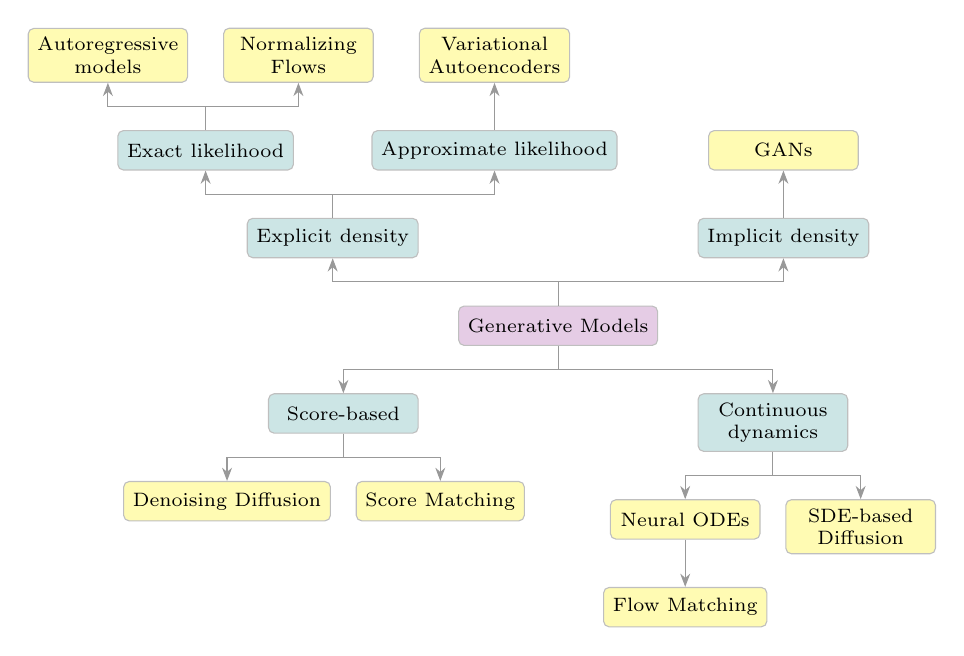
\begin{tikzpicture}[
    scale=1.0, transform shape,
    node distance=0.6cm and 0.3cm,
    box/.style={
        rectangle, 
        draw=gray!50, 
        rounded corners=2pt, 
        minimum width=1.9cm, 
        minimum height=0.5cm, 
        align=center, 
        font=\scriptsize, 
        line width=0.4pt
    },
    root/.style={box, fill=violet!20},
    category/.style={box, fill=teal!20},
    model/.style={box, fill=yellow!30},
    arrow/.style={-Stealth, draw=gray!80, line width=0.4pt}
]

    % --- CENTRAL ROOT ---
    \node[root] (root) {Generative Models};

    % --- UPPER BRANCHES (SWAPPED) ---
    % Tier 1: Explicit (Left) and Implicit (Right)
    \node[category, above left=0.6cm and 0.5cm of root] (explicit) {Explicit density};
    \node[category, above right=0.6cm and 0.5cm of root] (implicit) {Implicit density};

    % Tier 2 (Left side: Likelihoods)
    \node[category, above left=0.6cm and -0.6cm of explicit] (exact) {Exact likelihood};
    \node[category, above right=0.6cm and -0.6cm of explicit] (approx) {Approximate likelihood};

    % Tier 2 (Right side: GANs)
    \node[model, above=0.6cm of implicit] (gans) {GANs};

    % Tier 3 (Final Models Up)
    \node[model, above left=0.6cm and -0.9cm of exact] (ar) {Autoregressive \\ models};
    \node[model, above right=0.6cm and -0.9cm of exact] (nf) {Normalizing \\ Flows};
    \node[model, above=0.6cm of approx] (vae) {Variational \\ Autoencoders};

    % --- LOWER BRANCHES ---
    % Tier 1: Score-based and Continuous
    \node[category, below left=0.6cm and 0.5cm of root] (score) {Score-based};
    \node[category, below right=0.6cm and 0.5cm of root] (cont) {Continuous \\ dynamics};

    % Tier 2 (Score Models)
    \node[model, below left=0.6cm and -0.8cm of score] (ddpm) {Denoising Diffusion};
    \node[model, below right=0.6cm and -0.8cm of score] (sm) {Score Matching};

    % Tier 2 (Continuous Models)
    \node[model, below left=0.6cm and -0.8cm of cont] (node) {Neural ODEs};
    \node[model, below right=0.6cm and -0.8cm of cont] (sde) {SDE-based \\ Diffusion};

    % Tier 3 (Flow Matching)
    \node[model, below=0.6cm of node] (fm) {Flow Matching};

    % --- CONNECTIONS ---
    % Root to Tier 1
    \draw[arrow] (root.north) -- ++(0,0.3) -| (explicit.south);
    \draw[arrow] (root.north) -- ++(0,0.3) -| (implicit.south);
    \draw[arrow] (root.south) -- ++(0,-0.3) -| (score.north);
    \draw[arrow] (root.south) -- ++(0,-0.3) -| (cont.north);

    % Explicit side connections
    \draw[arrow] (explicit.north) -- ++(0,0.3) -| (exact.south);
    \draw[arrow] (explicit.north) -- ++(0,0.3) -| (approx.south);
    \draw[arrow] (exact.north) -- ++(0,0.3) -| (ar.south);
    \draw[arrow] (exact.north) -- ++(0,0.3) -| (nf.south);
    \draw[arrow] (approx.north) -- (vae.south);

    % Implicit side connection
    \draw[arrow] (implicit.north) -- (gans.south);

    % Score side connections
    \draw[arrow] (score.south) -- ++(0,-0.3) -| (ddpm.north);
    \draw[arrow] (score.south) -- ++(0,-0.3) -| (sm.north);

    % Continuous side connections
    \draw[arrow] (cont.south) -- ++(0,-0.3) -| (node.north);
    \draw[arrow] (cont.south) -- ++(0,-0.3) -| (sde.north);
    \draw[arrow] (node.south) -- (fm.north);

\end{tikzpicture}     % Generative models taxonomy diagram

\createdgmtitle{13}

%--------------------------------------------------------------------------------
\begin{document}
%--------------------------------------------------------------------------------
\begin{frame}[noframenumbering,plain]
\titlepage
	\resetonslide
\end{frame}
%=======
\begin{frame}{Recap of Previous Lecture}
	\myfootnotewithlink{https://arxiv.org/abs/2302.00482}{Tong A., et al. Improving and Generalizing Flow-Based Generative Models with Minibatch Optimal Transport, 2023}
	\begin{block}{Flow Matching (FM)}
		\vspace{-0.5cm}
		\[
			\bbE_{t \sim U[0, 1]} \bbE_{\bx \sim p_t(\bx)}\left\| \bff(\bx, t) - \bff_{\btheta}(\bx, t) \right\|^2 \rightarrow \min_{\btheta}
		\]
		\vspace{-0.5cm}
	\end{block}
	\begin{block}{Conditional Flow Matching (CFM)}
		\vspace{-0.5cm}
		\[
			\bbE_{t \sim U[0, 1]} \bbE_{\bz \sim p(\bz)} \bbE_{\bx \sim p_t(\bx | \bz)}\left\| \bff(\bx, \bz, t) - \bff_{\btheta}(\bx, t) \right\|^2 \rightarrow \min_{\btheta}
		\]
		\vspace{-0.7cm}
	\end{block}
	\begin{block}{Theorem}
		If $\text{supp}(p_t(\bx)) = \bbR^m$, then the optimal value of the FM objective equals the optimum for CFM.
	\end{block}
	\vspace{-0.3cm}
	\begin{figure}
		\centering
		\includegraphics[width=0.8\linewidth]{figs/multiple_dynamics}
	\end{figure}
\end{frame}
%=======
\begin{frame}{Recap of Previous Lecture}
    \myfootnotewithlink{https://dl.heeere.com/conditional-flow-matching/blog/conditional-flow-matching}{image credit: A Visual Dive into Conditional Flow Matching}
	\begin{figure}
		\centering
		\includegraphics[width=0.7\linewidth]{figs/cfm_uncond_to_cond}
	\end{figure}
	\vspace{-0.3cm}
	\begin{block}{Constraints}
		\vspace{-0.3cm}
		\[
			p(\bx) = \cN(0, \bI) = \bbE_{p(\bz)} p_0(\bx | \bz); \quad \pd(\bx) = \bbE_{p(\bz)} p_1(\bx | \bz).
		\]
		\vspace{-0.5cm}
	\end{block}
	\begin{itemize}
		\item How should we choose the conditioning latent variable $\bz$?
		\item How can we define $p_t(\bx | \bz)$ so that it meets the constraints?
	\end{itemize}
	\begin{block}{Gaussian Conditional Probability Path}
		\vspace{-0.3cm}
		\[
			p_t(\bx | \bz) = \cN\left(\bmu_t(\bz), \bsigma_t^2(\bz)\right)
		\]
		\[
			\bx_t = \bmu_t(\bz) + \bsigma_t(\bz) \odot \bx_0, \quad {\color{violet} \bx_0 \sim p_0(\bx) = \cN(0, \bI)}
		\]
	\end{block}
\end{frame}
%=======
\begin{frame}{Recap of Previous Lecture}
    \myfootnotewithlink{https://arxiv.org/abs/2210.02747}{Lipman Y., et al. Flow Matching for Generative Modeling, 2022}
	\begin{block}{Gaussian Conditional Probability Path}
		\vspace{-0.3cm}
		\[
			p_t(\bx | \bz) = \cN\left(\bmu_t(\bz), \bsigma_t^2(\bz)\right); \quad \bx_t = \bmu_t(\bz) + \bsigma_t(\bz) \odot \bx_0
		\]
		\vspace{-0.3cm}
		\[
			\bff(\bx, \bz, t) =  \bmu_t'(\bz) + \frac{\bsigma_t'(\bz)}{\bsigma_t(\bz)} \odot (\bx - \bmu_t(\bz))
		\]
		\vspace{-0.3cm}
	\end{block}
	\begin{block}{Conditioning Latent Variable}
		Let’s choose $\bz = \bx_1$. Then $p(\bz) = p_1(\bx_1)$.
		\[
			p_t(\bx) = \int p_t(\bx | \bx_1) p_1(\bx_1) d \bx_1
		\]
		\vspace{-0.5cm}
	\end{block}
	We must ensure the boundary constraints:
	\[
		\begin{cases}
			p(\bx) = \bbE_{p(\bz)} p_0(\bx | \bz); {\color{gray}(= \cN(0, \bI))} \\
			\pd(\bx) = \bbE_{p(\bz)} p_1(\bx | \bz).
		\end{cases}
		\quad \Rightarrow \quad 
		\begin{cases}
			p_0(\bx | \bx_1) = \cN(0, \bI); \\
			p_1(\bx | \bx_1) = \delta(\bx - \bx_1).
		\end{cases}
	\]
	\vspace{-0.3cm}
\end{frame}
%=======
\begin{frame}{Recap of Previous Lecture}
    \myfootnotewithlink{https://dl.heeere.com/conditional-flow-matching/blog/conditional-flow-matching}{image credit: A Visual Dive into Conditional Flow Matching}
	\[
		p_0(\bx | \bx_1) = \cN(0, \bI); \quad p_1(\bx | \bx_1) = \delta(\bx - \bx_1).
	\]
	
	\begin{block}{Gaussian Conditional Probability Path}
		\vspace{-0.5cm}
		\[
			p_t(\bx | \bx_1) = \cN\left(\bmu_t(\bx_1), \bsigma_t^2(\bx_1)\right); \quad \bx_t = \bmu_t(\bx_1) +  \bsigma_t(\bx_1) \odot \bx_0.
		\]
		\vspace{-0.6cm}
	\end{block}
	Let’s consider straight conditional paths:	
	\[
		\begin{cases}
			\bmu_t(\bx_1) = t \bx_1; \\
			\bsigma_t(\bx_1) = 1 - t.
		\end{cases}
		\quad \Rightarrow \quad 
		\begin{cases}
			p_t(\bx | \bx_1) = \cN\left(t \bx_1, (1-t)^2 \bI\right); \\
		 	\bx_t = t \bx_1 + (1 - t) \bx_0. 
	 \end{cases}
	\]
	\vspace{-0.3cm}
	\begin{figure}
		\centering
		\includegraphics[width=\linewidth]{figs/conical_paths}
	\end{figure}
\end{frame}
%=======
\begin{frame}{Recap of Previous Lecture}
	\myfootnotewithlink{https://mlg.eng.cam.ac.uk/blog/2024/01/20/flow-matching.html}{image credit: https://mlg.eng.cam.ac.uk/blog/2024/01/20/flow-matching.html}
	\[
		p_t(\bx | \bx_1) = \cN\left(t \bx_1, (1-t)^2 \bI\right); \quad {\color{teal}\bx_t = t \bx_1 + (1 - t) \bx_0}
	\]
	\vspace{-0.3cm}
	\[
		\bff(\bx_t, \bx_1, t) = \frac{\bx_1 - \bx_t}{1-t} = \bx_1 - \bx_0
	\]
	\vspace{-0.7cm}
	\begin{multline*}
		\bbE_{\bz \sim p(\bz)} \bbE_{\bx \sim p_t(\bx | \bz)}\left\| \bff(\bx, \bz, t) - \bff_{\btheta}(\bx, t) \right\|^2
		 = \\ = \bbE_{\bx_1 \sim \pd(\bx)} \bbE_{\bx_0 \sim \cN(0, \bI)}\left\| (\bx_1 - \bx_0) - \bff_{\btheta}\left(t \bx_1 + (1 - t) \bx_0, t\right) \right\|^2
	\end{multline*}
	\vspace{-0.7cm}
	\begin{itemize}
		\item $\bff(\bx_t, \bx_1, t)$ defines straight lines between $\pd(\bx)$ and $\cN(0, \bI)$.
		\item The \textbf{marginal} path $p_t(\bx)$ does not give straight lines.
	\end{itemize}
	\vspace{-0.5cm}
	\begin{minipage}[t]{0.5\columnwidth}
			\begin{figure}
				\centering
				\includegraphics[width=\linewidth]{figs/g2g-vector-field-samples-cond}
			\end{figure}
		\end{minipage}%
		\begin{minipage}[t]{0.5\columnwidth}
			\begin{figure}
				\centering
				\includegraphics[width=\linewidth]{figs/g2g-forward_samples}
			\end{figure}
	\end{minipage}
\end{frame}
%=======
\begin{frame}{Recap of Previous Lecture}
	\myfootnotewithlink{https://arxiv.org/abs/2210.02747}{Lipman Y., et al. Flow Matching for Generative Modeling, 2022}
	\vspace{-0.3cm}
	\[
	 \bbE_{t \sim U[0, 1]} \bbE_{\bx_1 \sim \pd(\bx)} \bbE_{\bx_0 \sim \cN(0, \bI)}\left\| (\bx_1 - \bx_0) - \bff_{\btheta}(\bx_t, t) \right\|^2  \rightarrow \min_{\btheta}
	\]
	\begin{block}{Training}
		\begin{enumerate}
			\item Sample $\bx_1 \sim \pd(\bx)$.
			\item Sample time $t \sim U[0, 1]$ and $\bx_0 \sim \cN(0, \bI)$.
			\item Obtain the noisy image $\bx_t = t \bx_1 + (1 - t) \bx_0$.
			\item Compute the loss $ \cL = \left\| (\bx_1 - \bx_0) - \bff_{\btheta}(\bx_t, t) \right\|^2 $.
		\end{enumerate}
	\end{block}
	\vspace{-0.3cm}
	\begin{block}{Sampling}
		\begin{enumerate}
			\item Sample $\bx_0 \sim \cN(0, \bI)$.
			\item Solve the ODE to obtain $\bx_1$:
			\[
				\bx_1 = \texttt{ODESolve}_f(\bx_0, \btheta, t_0=0, t_1=1)
			\]
		\end{enumerate}
	\end{block}
\end{frame}
%=======
\begin{frame}{Recap of Previous Lecture}
	\myfootnotewithlink{https://dl.heeere.com/conditional-flow-matching/blog/conditional-flow-matching}{image credit: A Visual Dive into Conditional Flow Matching}
	
	Let us choose $\bz = (\bx_0, \bx_1)$. Then $p(\bz) = p (\bx_0, \bx_1) = p_0(\bx_0) p_1(\bx_1)$.
	\[
		p_0(\bx | \bx_0, \bx_1) = \delta(\bx - \bx_0); \quad p_1(\bx | \bx_0, \bx_1) = \delta(\bx - \bx_1)
	\]
	\vspace{-0.5cm}
	\begin{block}{Gaussian Conditional Probability Path}
		\vspace{-0.5cm}
		{\small
		\[
			p_t(\bx | \bx_0, \bx_1) = \cN\left(\bmu_t(\bx_0, \bx_1), \bsigma_t^2(\bx_0, \bx_1)\right); \quad \bx_t = \bmu_t(\bx_0, \bx_1) +  \bsigma_t(\bx_0, \bx_1) \odot \bepsilon
		\]
		}
		\vspace{-0.7cm}
	\end{block}
	Let's consider straight conditional paths:	
	\[
		\bmu_t(\bx_1) = t \bx_1 + (1 - t) \bx_0 \quad
		\bsigma_t(\bx_1) = \epsilon
	\]
	\vspace{-0.7cm}
	\begin{figure}
		\centering
		\includegraphics[width=\linewidth]{figs/linear_paths}
	\end{figure}
\end{frame}
%=======
\begin{frame}{Recap of Previous Lecture}
	\myfootnotewithlink{https://arxiv.org/abs/2302.00482}{Tong A., et al. Improving and Generalizing Flow-Based Generative Models with Minibatch Optimal Transport, 2023}
	\begin{minipage}[t]{0.5\columnwidth}
		\textbf{Endpoint conditioning}
		\begin{align*}
			\bz & = \bx_1 \\
			p_t(\bx | \bx_1) &= \cN\left(t \bx_1, (1-t)^2 \bI\right) \\
			\bx_t &= t \bx_1 + (1 - t) \bx_0 
		\end{align*}
	\end{minipage}%
	\begin{minipage}[t]{0.5\columnwidth}
		\textbf{Pair conditioning}
		\begin{align*}
			\bz & = (\bx_0, \bx_1) \\
			p_t(\bx | \bx_0, \bx_1) &= \cN\left(t \bx_1 + (1 - t) \bx_0, \epsilon^2 \bI\right) \\
			\bx_t &= t \bx_1 + (1 - t) \bx_0
		\end{align*}
	\end{minipage}
	\begin{figure}
		\centering
		\includegraphics[width=0.8\linewidth]{figs/compare_conditionings}
	\end{figure}
\end{frame}
%=======
\begin{frame}{Recap of Previous Lecture}
	\myfootnotewithlink{https://arxiv.org/abs/2210.02747}{Lipman Y., et al. Flow Matching for Generative Modeling, 2022}
	\begin{itemize}
		\item This conditioning allows us to transport any distribution $p_0(\bx)$ to any distribution $p_1(\bx)$.
		\item It's possible to apply this approach to paired tasks, e.g., style transfer.
	\end{itemize}
	\begin{block}{Training Procedure}
		\begin{enumerate}
			\item Sample $(\bx_0, \bx_1) \sim p(\bx_0, \bx_1)$.
			\item Sample time $t \sim U[0, 1]$.
			\item Compute the noisy image $\bx_t = t \bx_1 + (1 - t) \bx_0$.
			\item Compute the loss $ \cL = \left\| (\bx_1 - \bx_0) - \bff_{\btheta}(\bx_t, t) \right\|^2 $.
		\end{enumerate}
	\end{block}
	\vspace{-0.3cm}
	\begin{block}{Sampling}
		\begin{enumerate}
			\item Sample $\bx_0 \sim p_0(\bx)$.
							\item Solve the ODE to obtain $\bx_1$:
			\[
				\bx_1 = \texttt{ODESolve}_f(\bx_0, \btheta, t_0=0, t_1=1)
			\]
		\end{enumerate}
	\end{block}
\end{frame}
%=======
\begin{frame}{Outline}
	\tableofcontents
\end{frame}
%=======
\section{Link between Flow Matching and Score-Based Models}
%=======
\begin{frame}{Score-Based Generative Models through SDEs}
	\myfootnotewithlink{https://arxiv.org/abs/2210.02747}{Lipman Y., et al. Flow Matching for Generative Modeling, 2022}
	\vspace{-0.3cm}
	\begin{block}{Training}
		\vspace{-0.7cm}
		\[
			\bbE_{\pd(\bx(0))} \bbE_{t \sim U[0, 1]} \bbE_{q(\bx(t) | \bx(0))}\bigl\| \bs_{\btheta}(\bx(t), t) - {\color{teal}\nabla_{\bx(t)} \log q(\bx(t) | \bx(0))} \bigr\|^2_2 
		\]
		\vspace{-0.5cm}
	\end{block}
	\eqpause
	\begin{block}{Variance Exploding SDE (NCSN)}
		\vspace{-0.3cm}
		\[
			q(\bx(t) | \bx(0)) = \cN\left(\bx(0), \left[\sigma^2(t) - \sigma^2(0)\right] \cdot \bI\right), \quad \sigma(0) =0
		\]
		\vspace{-0.5cm}
	\end{block}
	\begin{block}{Variance Preserving SDE (DDPM)}
		\vspace{-0.5cm}
		\[
			q(\bx(t) | \bx(0)) = \cN\left(\bx(0) \alpha(t), \left(1 - \alpha(t)^2\right) \cdot \bI\right); \quad \alpha(t) = e^{-\frac{1}{2} \int_0^t \beta(s) ds}
		\]
		\vspace{-0.5cm}
	\end{block}
	\eqpause
	Flow matching uses reverse time direction:
	\[
		p_t(\bx| \bx_1) = q_{1-t}(\bx| \bx_0=\bx_1)
	\]
\end{frame}
%=======
\begin{frame}{Score-Based Generative Models through SDEs}
	\[
		p_t(\bx| \bx_1) = q_{1-t}(\bx| \bx_0=\bx_1)
	\]
	\[
		\textbf{VE (NCSN): } p_t(\bx | \bx_1) = \cN\left(\bx_1, \sigma^2_{1-t} \cdot \bI\right)
	\]
	\vspace{-0.5cm}
	\[
		\textbf{VP (DDPM): } p_t(\bx | \bx_1) = \cN\left(\alpha_{1-t} \bx_1, \left(1 - \alpha_{1-t}^2\right) \cdot \bI\right)
	\]
	\vspace{-0.5cm}
	\eqpause
	\begin{block}{Flow Matching Probability Path}
		\vspace{-0.3cm}
		\[
			p_t(\bx | \bx_1) = \cN\left(t \bx_1, (1-t)^2 \bI\right); \quad \bff(\bx_t, \bx_1, t) = \frac{\bx_1  - \bx_t}{1-t}
		\]
		\vspace{-0.3cm}
		\[
	 		\frac{d\bx_t}{dt} = \bff(\bx_t, \bx_1, t) =  \bmu_t'(\bx_1) + \frac{\bsigma_t'(\bx_1)}{\bsigma_t(\bx_1)} \odot (\bx_t - \bmu_t(\bx_1))
		\]
	\end{block}
	\eqpause
	Let's derive the conditional vector fields for VE (NCSN) and VP (DDPM).
\end{frame}
%=======
\begin{frame}{Flow Matching vs. Score-Based SDE Models}
	\myfootnotewithlink{https://arxiv.org/abs/2210.02747}{Lipman Y., et al. Flow Matching for Generative Modeling, 2022}
	\[
		\frac{d\bx_t}{dt} = \bff(\bx_t, \bx_1, t) =  \bmu_t'(\bx_1) + \frac{\bsigma_t'(\bx_1)}{\bsigma_t(\bx_1)} \odot (\bx_t - \bmu_t(\bx_1))
	\]
	\eqpause
	\begin{block}{Variance Exploding SDE Probability Path}
		\vspace{-0.5cm}
		\[
				p_t(\bx | \bx_1) = \cN\left(\bx_1, \sigma^2_{1-t}  \bI\right) \quad \Rightarrow \quad 
				\bff(\bx_t, \bx_1, t) = - \frac{\sigma'_{1-t}}{\sigma_{1-t}} (\bx_t - \bx_1)
		\]
		\vspace{-0.3cm}
	\end{block}
	\eqpause
	\begin{block}{Variance Preserving SDE Probability Path}
		\vspace{-0.5cm}
		{\small
		\[
			p_t(\bx | \bx_1) = \cN\left(\alpha_{1-t}  \bx_1, (1 - \alpha^2_{1-t})  \bI \right)  \, \Rightarrow \, 
		\bff(\bx_t, \bx_1, t) = \frac{\alpha'_{1-t}}{1 - \alpha^2_{1-t}}\cdot \left(\alpha_{1-t}  \bx_t - \bx_1\right)
		\]
		}
	\end{block}
	Thus, VE/VP SDE models correspond to particular choices of the Gaussian probability path within the flow matching framework.
\end{frame}
%=======
\begin{frame}{Flow Matching vs. Score-Based SDE Models}
	\myfootnotewithlink{https://arxiv.org/abs/2210.02747}{Lipman Y., et al. Flow Matching for Generative Modeling, 2022}
	\begin{block}{Trajectories}
		\vspace{-0.3cm}
		\begin{figure}
			\centering
			\includegraphics[width=0.6\linewidth]{figs/trajectories}
		\end{figure}
		\vspace{-0.3cm}
	\end{block}
	\eqpause
	\begin{figure}
		\centering
		\includegraphics[width=\linewidth]{figs/2d-generation}
	\end{figure}
\end{frame}
%=======
\section{Discrete Diffusion Models}
%=======
\begin{frame}{Discrete or Continuous Diffusion Models?}
	\textbf{Reminder:} Diffusion models define a forward corruption process and a reverse denoising process.
	Previously, we studied diffusion models with continuous states $\bx(t) \in \mathbb{R}^m$.
	\begin{block}{Continuous state space}
		\begin{itemize}
			\item \textbf{Discrete time} $t \in \{0,1,\ldots,T\}$ $\;\Rightarrow\;$ \textbf{DDPM / NCSN}.
			\item \textbf{Continuous time} $t \in [0,1]$ $\;\Rightarrow\;$ \textbf{Score-based SDE models}.
		\end{itemize}
	\end{block}
	\eqpause
	Now we turn to diffusion over discrete-value states $\bx(t) \in \{1, \dots, K\}^m$.
	\begin{block}{Discrete state space}
		\begin{itemize}
			\item \textbf{Discrete time} $t \in \{0,1,\ldots,T\}$.
			\item \textbf{Continuous time} $t \in [0,1]$.
		\end{itemize}
	\end{block}
	Let's discuss why we need discrete diffusion models.
\end{frame}
%=======
\begin{frame}{Why Discrete Diffusion Models?}
	\myfootnotewithlink{https://aaronlou.com/blog/2024/discrete-diffusion/}{https://aaronlou.com/blog/2024/discrete-diffusion/}
	While autoregressive (AR) models dominate discrete-data domains (e.g., text or sequences), they have fundamental limitations.
	\eqpause
	\begin{block}{Key advantages of discrete diffusion}
		\begin{itemize}
			\item \textbf{Parallel generation:} diffusion enables sampling all tokens simultaneously, unlike AR’s strictly left-to-right process. 
			\eqpause
			\item \textbf{Flexible infilling:}. diffusion can mask arbitrary parts of a sequence and reconstruct them, rather than generating only from prefix to suffix.
			\eqpause 
			\item \textbf{Robustness:} diffusion avoids the "exposure bias" caused by teacher forcing in AR training.
			\eqpause
			\item \textbf{Unified framework:} diffusion generalizes naturally to discrete domains that do not suit continuous Gaussian noise.
		\end{itemize}
	\end{block}
\end{frame}
%=======
\begin{frame}{2025 – Big Bang of Discrete Diffusion Models}
	\myfootnotewithlink{https://arxiv.org/abs/2506.17298}{Khanna S. et al. Mercury: Ultra-fast language models based on diffusion, 2025.}
	\begin{figure}
		\includegraphics[width=\linewidth]{figs/mercury}
	\end{figure}
\end{frame}
%=======
\subsection{Forward Discrete Process}
%=======
\begin{frame}{Forward Discrete Process}
	\myfootnotewithlink{https://arxiv.org/abs/2107.03006}{Austin J. et al. Structured denoising diffusion models in discrete state-spaces, 2021.}
	\begin{block}{Continuous Diffusion Markov Chain}
		In continuous diffusion, the forward Markov chain is defined by progressively corrupting data with Gaussian noise:
		\[
			q(\bx_t|\bx_{t-1}) = \mathcal{N}(\sqrt{1-\beta_t}\bx_{t-1}, \beta_t \bI).
		\]
	\end{block}
	\eqpause
	\vspace{-0.3cm}
	\begin{block}{Discrete Diffusion Markov Chain}
		For discrete data, we instead define a Markov chain over categorical states:
		\[
			q(\bx_t|\bx_{t-1}) = \Cat(\bQ_t\bx_{t-1}),
		\]
	\end{block}
	\vspace{-0.3cm}
	\eqpause
	\begin{itemize}
		\item Each $\bx_t \in \{0,1\}^K$ is a \textbf{one-hot vector} encoding the categorical state (it is just one token).
		\item What is the transition matrix $\bQ_t$?
	\end{itemize}
\end{frame}
%=======
\begin{frame}{Forward Process over Time}
	\myfootnotewithlink{https://arxiv.org/abs/2107.03006}{Austin J. et al. Structured denoising diffusion models in discrete state-spaces, 2021.}
	\begin{block}{Transition Matrix}
		$\bQ_t \in [0,1]^{K \times K}$ is a \textbf{transition matrix} where each column gives transition probabilities from one state to all others, and columns sum to 1:
		\vspace{-0.5cm}
		\[
			[\bQ_t]_{ij} = q(x_t = i | x_{t-1} = j),
			\qquad
			\sum_{i=1}^K [\bQ_t]_{ij} = 1.
		\]
		\vspace{-0.7cm}
	\end{block}
	\eqpause
	\begin{itemize}
		\item The forward diffusion gradually destroys information through repeated random transitions.
		\eqpause
		\item Applying the transition $t$ times yields the marginal distribution:
			\[
				q(\bx_t|\bx_0) = \Cat(\bQ_{1:t}\bx_0),
				\qquad
				\bQ_{1:t} = \bQ_t \bQ_{t-1}\cdots\bQ_1.
			\]
		\eqpause
		\vspace{-0.7cm}
		\item As $t \to T$, the process drives the data toward a stationary distribution.
		\eqpause
		\item We design the transition matrices $\bQ_t$ to achieve this behavior.
	\end{itemize}
\end{frame}
%=======
\begin{frame}{Transition Matrix}
	\myfootnotewithlink{https://arxiv.org/abs/2107.03006}{Austin J. et al. Structured denoising diffusion models in discrete state-spaces, 2021.}
	\begin{itemize}
		\item The choice of $\bQ_t$ determines how information is erased and what the stationary distribution becomes.
		\eqpause
		\item $\bQ_t$ and $\bQ_{1:t}$ should be easy to compute for each $t$.
	\end{itemize}
	\eqpause
	\begin{block}{Common choices}
		\begin{itemize}
			\item \textbf{Uniform diffusion}
			\[
				\bQ_t = (1 - \beta_t) \bI + \beta_t \bU,
				\qquad
				\mathbf{U}_{ij} = \tfrac{1}{K}.
			\]
			Each token is replaced by a uniformly random symbol with probability $\beta_t$.
			The stationary distribution is uniform noise.
			\eqpause
			\item \textbf{Absorbing diffusion}
			\[
				\bQ_t = (1-\beta_t)\bI + \beta_t\, \mathbf{e}_m \mathbf{1}^\top.
			\]
			Tokens are gradually replaced by a special mask $m$;
			the stationary distribution is fully masked.
		\end{itemize}
	\end{block}
\end{frame}
%=======
\begin{frame}{Transition Matrix}
	\[
		q(\bx_t|\bx_0) = \Cat(\bQ_{1:t}\bx_0),
		\qquad
		\bQ_{1:t} = \bQ_t \bQ_{t-1} \cdots \bQ_1.
	\]
	\eqpause
	\begin{block}{Uniform Diffusion}
		\[
			\bQ_t = (1-\beta_t)\bI + \beta_t \mathbf{U},
			\qquad
			\mathbf{U}_{ij} = \tfrac{1}{K}.
		\]
		\[
			\bQ_{1:t} = \bar\alpha_t\bI + (1 - \bar\alpha_t) \mathbf{U},
			\quad
			\bar\alpha_t = \prod_{s=1}^t (1-\beta_s).
		\]
		\eqpause
		\begin{itemize}
			\item Each token retains its original value with prob.~$\bar\alpha_t$.
			\item It becomes uniformly random with prob.~$(1 - \bar\alpha_t)$.
			\item As $t \to T$, the process converges to the stationary uniform distribution.
		\end{itemize}
	\end{block}
\end{frame}
%=======
\begin{frame}{Transition Matrix}
	\myfootnotewithlink{https://arxiv.org/abs/2107.03006}{Austin J. et al., Structured denoising diffusion models in discrete state-spaces, 2021.}

	\begin{block}{Absorbing Diffusion}
		\[
			\bQ_t = (1-\beta_t)\bI + \beta_t\, \mathbf{e}_m \mathbf{1}^\top,
		\]
		\[
			\bQ_{1:t} = \bar\alpha_t\,\bI + (1-\bar\alpha_t)\,\mathbf{e}_m \mathbf{1}^\top,
			\qquad
			\bar\alpha_t = \prod_{s=1}^t (1-\beta_s).
		\]
		\eqpause
		\begin{itemize}
			\item Each token retains its original value with prob.~$\bar\alpha_t$.
			\item It becomes $\mathbf{e}_m$ with prob.~$(1 - \bar\alpha_t)$.
			\item As $t \to T$, all tokens converge to the mask state: $q(\bx_T) \approx \Cat(\mathbf{e}_m)$.
			\item This makes the process analogous to \textbf{masked language modeling}.
		\end{itemize}
	\end{block}
\end{frame}
%=======
\begin{frame}{Uniform vs. Absorbing Transition Matrix}
	\myfootnotewithlink{https://arxiv.org/abs/2107.03006}{Austin J. et al., Structured denoising diffusion models in discrete state-spaces, 2021.}
	\begin{table}[h!]
		\centering
		\small
		\begin{tabular}{lcc}
			\toprule
			\textbf{Aspect} & \textbf{Uniform Diffusion} & \textbf{Absorbing Diffusion} \\
			\midrule
			$\bQ_t$
				& $(1-\beta_t)\bI + \beta_t \mathbf{U}$ 
				& $(1-\beta_t)\bI + \beta_t \mathbf{e}_m\mathbf{1}^\top$ \\[4pt]
			$\bQ_{1:t}$
				& $\bar\alpha_t \bI + (1-\bar\alpha_t)\mathbf{U}$
				& $\bar\alpha_t \bI + (1-\bar\alpha_t)\mathbf{e}_m\mathbf{1}^\top$ \\[4pt]
			$\bQ_{1:\infty}$
				& $\mathbf{U}$
				& $\Cat(\mathbf{e}_m)$ \\[4pt]
			Interpretation
				& Random replacement
				& Gradual masking of tokens \\[4pt]
			Application
				& Image diffusion
				& Text diffusion $\approx$ Masked LM \\[4pt]
			\bottomrule
		\end{tabular}
	\end{table}
	\eqpause
	\begin{block}{Observation}
		Both schemes gradually destroy information, but differ in their stationary limit.
		Absorbing diffusion bridges diffusion and masked-language-model objectives.
	\end{block}
\end{frame}
%=======
\subsection{Reverse Discrete Diffusion}
%=======
\begin{frame}{Posterior of the Forward Process}
	\myfootnotewithlink{https://arxiv.org/abs/2107.03006}{Austin J. et al., Structured denoising diffusion models in discrete state-spaces, 2021.}
	\begin{block}{ELBO}
		\vspace{-0.7cm}
		\begin{multline*}
            \cL_{\bphi, \btheta}(\bx) =  {\color{olive}\bbE_{q(\bx_1 | \bx_0)} \log \pt(\bx_0 | \bx_1)} - {\color{violet}\KL\bigl(q(\bx_T | \bx_0) \| p(\bx_T)\bigr)} - \\
            - {\color{teal}\sum_{t=2}^\top \underbrace{ \bbE_{q(\bx_t | \bx_0)} \KL \bigl(q(\bx_{t-1} | \bx_t, \bx_0) \| \pt(\bx_{t-1} | \bx_t)\bigr)}_{\cL_t}}
        \end{multline*}
		\vspace{-0.7cm}
	\end{block}
	\eqpause
	\begin{itemize}
		\item Conditioned reverse distribution $q(\bx_{t-1} | \bx_t, \bx_0)$ played crucial role in the continuous-state diffusion model.
		\item It shows the probability of a previous state given the noisy state $\bx_t$ and the original clean data $\bx_0$.
	\end{itemize}
	\eqpause
	\begin{block}{Discrete conditioned reverse distribution}
		\vspace{-0.7cm}
		\begin{align*}
			q(\bx_{t-1} | \bx_t, \bx_0)
			&= \frac{q(\bx_t | \bx_{t-1}, \bx_0)\, q(\bx_{t-1} | \bx_0)}
			        {q(\bx_t | \bx_0)} \\
			&= \frac{\Cat(\bQ_t) \cdot \Cat(\bQ_{1:t-1})}{\Cat(\bQ_{1:t})}.
		\end{align*}
	\end{block}
\end{frame}
%=======
\begin{frame}{Posterior of the Forward Process}
	\myfootnotewithlink{https://arxiv.org/abs/2107.03006}{Austin J. et al., Structured denoising diffusion models in discrete state-spaces, 2021.}
	\begin{block}{Discrete conditioned reverse distribution}
		\[
			q(\bx_{t-1} | \bx_t, \bx_0)
			= \Cat\left(\frac{\bQ_t \bx_t \odot \bQ_{1:t-1} \bx_0}{\bx_t^{\top}\bQ_{1:t}\bx_0}\right).
		\]
		\vspace{-0.3cm}
	\end{block}
	\eqpause
	Recall the ELBO term
	\[
		\cL_t
		= \bbE_{q(\bx_t | \bx_0)}
		\KL\bigl(q(\bx_{t-1} | \bx_t, \bx_0) \,\|\, \pt(\bx_{t-1} | \bx_t)\bigr),
	\]
	\eqpause
	\vspace{-0.5cm}
	\begin{itemize}
		\item Both $q(\bx_{t-1} | \bx_t, \bx_0)$ and $q(\bx_t | \bx_0)$ are known analytically from the forward process.
		\item The reverse process $\pt(\bx_{t-1} | \bx_t)$ is a learned categorical distribution:
		\[
			\pt(\bx_{t-1} | \bx_t) = \Cat\bigl( \bpi_{\btheta}(\bx_t, t) \bigr),
		\]
		where $\bpi_{\btheta}$ is a neural network.
	\end{itemize}
\end{frame}
%=======
\begin{frame}{Discrete-time ELBO for Discrete Diffusion}
	\myfootnotewithlink{https://arxiv.org/abs/2107.03006}{Austin J. et al., Structured denoising diffusion models in discrete state-spaces, 2021.}

	\begin{block}{ELBO term}
		\vspace{-0.3cm}
		\[
			\cL_t
			= \bbE_{q(\bx_t | \bx_0)}
			\KL\bigl(q(\bx_{t-1} | \bx_t, \bx_0) \,\|\, \pt(\bx_{t-1} | \bx_t)\bigr).
		\]
		\vspace{-0.3cm}
	\end{block}
	\eqpause
	\begin{block}{Categorical KL}
		\vspace{-0.3cm}
		\[
			\KL\bigl(\Cat(\bq) \,\|\, \Cat(\bp)\bigr)
			= \sum_{k=1}^K q_k \log \frac{q_k}{p_k}
			= \Ent(\bq,\bp) - \Ent(\bq),
		\]
		\eqpause
		\begin{itemize}
			\item $\Ent\bigl(q(\bx_{t-1} | \bx_t, \bx_0)\bigr)$ is a constant w.r.t.~$\btheta$.
			\item $\Ent(\bq,\bp) = -\sum_k q_k \log p_k$ is a \textbf{cross-entropy loss}.
		\end{itemize}
	\end{block}
	\eqpause
	Therefore, minimizing $\cL_t$ w.r.t.~$\btheta$ is equivalent to minimizing
	\[
		\bbE_{q(\bx_t | \bx_0)}
		\Ent\Bigl(q(\bx_{t-1} | \bx_t, \bx_0),\, \pt(\bx_{t-1} | \bx_t)\Bigr).
	\]
\end{frame}
%=======
\begin{frame}{Summary}
	\begin{itemize}
		\item Diffusion and score-based models are special cases of the flow matching approach, but use curved trajectories.
		\vfill
		\item Diffusion approach has several key advantages over autoregressive approach.
		\vfill
		\item Forward discrete diffusion process defines Markov chain with discrete states.
		\vfill
		\item There are several ways to make it tractable (uniform / absorbing transitions).
		\vfill
		\item Reverse discrete diffusion process uses the variational approach to invert forward process.
		\vfill 
		\item Discrete-state ELBO for discrete diffusion is a cross-entropy loss. 
	\end{itemize}
\end{frame}
\end{document}